%%%%%%%%%%%%%%%%%%%%%%%%%%%%%%%%%%%%%%%%%%%%%%%%%%%%%%%%%%%%%%%%%%%%
% This was inspired by Ivan Griffin's work on a periodic table
% (http://www.texample.net/tikz/examples/author/ivan-griffin/)
% Back in 2015, I adapted/modified Ivan's periodic table to suit
% my needs for a chemistry class that I taught.
% What you find here is a complete 're-design.' so I am releasing
% the re-designed code with a new copyright license.
% Specifically, this code is distributed under the MIT open source
% license.
% Copyright 2019 Paul N. Danese
% Permission is hereby granted, free of charge, to any person
% obtaining a copy of this software and associated documentation
% files (the "Software"), to deal in the Software without
% restriction, including without limitation the rights to use,
% copy, modify, merge, publish, distribute, sublicense, and/or
% sell copies of the Software, and to permit persons to whom the
% Software is furnished to do so, subject to the following
% conditions:
% The above copyright notice and this permission notice shall
% be included in all copies or substantial portions of the Software.
% THE SOFTWARE IS PROVIDED "AS IS", WITHOUT WARRANTY OF ANY KIND,
% EXPRESS OR IMPLIED, INCLUDING BUT NOT LIMITED TO THE WARRANTIES OF
% MERCHANTABILITY, FITNESS FOR A PARTICULAR PURPOSE AND NONINFRINGEMENT.
% IN NO EVENT SHALL THE AUTHORS OR COPYRIGHT HOLDERS BE LIABLE FOR
% ANY CLAIM, DAMAGES OR OTHER LIABILITY, WHETHER IN AN ACTION OF
% CONTRACT, TORT OR OTHERWISE, ARISING FROM, OUT OF OR IN CONNECTION
% WITH THE SOFTWARE OR THE USE OR OTHER DEALINGS IN THE SOFTWARE.
%%%%%%%%%%%%%%%%%%%%%%%%%%%%%%%%%%%%%%%%%%%%%%%%%%%%%%%%%%%%%%%%%%%%
\documentclass[9pt]{article}
\usepackage{geometry}
\usepackage{ccicons}
\usepackage{chem}
\usepackage{chemmacros}
\usepackage{multicol}
\usepackage{siunitx}
\geometry{
    letterpaper,
    left=2mm,
    right=2mm,
    bottom=2mm,
    top=2mm
}
\usepackage{graphicx}
% creative commons icons
\usepackage{ccicons}
%%%%%%%%%%%%%%%%%%%%%%%%%%%%%%%%%%%
% url stuff                      %%
%%%%%%%%%%%%%%%%%%%%%%%%%%%%%%%%%%%
\usepackage{hyperref}
\hypersetup{% remove ugly boxes around url
    colorlinks,
    urlcolor={blue!80!black}
}
\urlstyle{same} % make url use the standard font

%%%%%%%%%%%%%%%%%%%%%%%%%%%%%%%%%%%
% tikz stuff                     %%
%%%%%%%%%%%%%%%%%%%%%%%%%%%%%%%%%%%
\usepackage{tikz} % the workhorse package here
\usepackage{pgfornament} % for the fancy corners and such
\usetikzlibrary{positioning,shapes}


%%%%%%%%%%%%%%%%%%%%%%%%%%%%%%%%%%%
% font stuff                     %%
%%%%%%%%%%%%%%%%%%%%%%%%%%%%%%%%%%%
\usepackage{fontspec} % I like fonts.
\setmainfont{Scala Pro}[Numbers={Proportional,Lining}]
\setsansfont{Scala Sans OT}[Numbers={Proportional,Lining}]


%%%%%%%%%%%%%%%%%%%%%%%%%%%%%%%%%%%
% color stuff                    %%
%%%%%%%%%%%%%%%%%%%%%%%%%%%%%%%%%%%
\definecolor{maroon}{HTML}{800000}
\definecolor{fancyyellow}{HTML}{FFFDE9}
\usepackage{pagecolor} % to color the page background (for extra fanciness)


%%%%%%%%%%%%%%%%%%%%%%%%%%%%%%%%%%%
% tikz styles                    %%
%%%%%%%%%%%%%%%%%%%%%%%%%%%%%%%%%%%
\tikzstyle{ebox} = [draw=black, thick,rectangle, minimum width=25mm,minimum height=25mm, node distance=25mm] % declares the features of each element box
\tikzstyle{Offsetter} = [ minimum width=24mm, minimum height=25mm, node distance=25mm] % declares features of an unseen box similar to ebox to provide a seed-point for the hydrogen box

% colors for different atomic blocks
\tikzstyle{Sblock} = [fill=cyan!10]
\tikzstyle{Pblock} = [fill=blue!10]
\tikzstyle{Dblock} = [fill=orange!10]
\tikzstyle{Fblock} = [fill=green!10]
\tikzstyle{Noblock} = [fill=gray!10]

% styles for the key and for details found at the bottom of the screen
\tikzstyle{KeysLabel} = [minimum height = 2.5cm, inner sep=0pt, text width = 7.5cm]
\tikzstyle{DetailsLabel} = [minimum height = 2.5cm, inner sep=0pt, text width = 35cm]
%%%%%%%%%%%%%%%%%%%%%%%%%%%%%%%%%%%%%%%%%%%%%%%%%%%%%%%%%%%%%%%%%%%
\newcommand{\moleculep}{\chemfig{
        O% 10
        =[:90]% 9
        (
        -[:30,,,1]OH% 11
        )
        -[:150]% 8
        (
        <:[:90,,,1]NH_2% 12
        )
        -[:210]% 7
        -[:150]% 4
        =^[:90]% 3
        -[:150]% 2
        =^[:210]% 1
        -[:270]% 6
        =^[:330]% 5
        (
        -[:30]% -> 4
        )
}}

\newcommand{\moleculeq}{\chemfig{
    O% 10
    =[:90]% 9
    (
    -[:150,,,2]HO% 11
    )
    -[:30]% 8
    (
    <[:90,,,1]NH_2% 12
    )
    -[:330]% 7
    -[:30]% 4
    =_[:90]% 3
    -[:30]% 2
    =_[:330]% 1
    -[:270]% 6
    =_[:210]% 5
    (
    -[:150]% -> 4
    )
}}

% this macro is used to add contents to each 'box' for each element
% parameter list is as follows:
%   #1: symbol
%   #2: element name
%   #3: atomic_number
%   #4: atomic_mass
%   #5: electronegativity (not used for 101 branch)
%   #6: shell occupied by 'last' ground-state electron (not used for 101 branch)
%   #7: subshell occupied by 'last' ground-state electron (not used for 101 branch)
\newcommand\periodicelement[7]{%
    \begin{minipage}{22mm}%
        \centering%
        \par\noindent\parbox[t]{.333\textwidth}{\raggedright\textsf{\phantom{#3}}}%
        \parbox[t]{.333\textwidth}{\centering\textsf{#3}}%
        \parbox[t]{.333\textwidth}{\raggedleft \textsf{\phantom{#6}\textit{\phantom{#7}}}}\par%
        \vspace*{0.5em}%
        {\Huge #1}\\%
        \vspace*{0.14em}%
        \textsf{#2}\\%
        #4\\%
\end{minipage}}%

% create a phantom endash to go in certain boxes that don't have or need a number
\newcommand{\pendash}{\phantom{\textendash}}
% This macro is primarily used to create asterisks that delineate the
% lanthanide and actinide series at the bottom of the table.
\newcommand{\offsetterbox}[9]{\node[name=#1, Offsetter, #8, #9] {\periodicelement{#1}{#2}{#3}{#4}{#5}{#6}{#7}};}

% name text position shading
\newcommand{\groupbox}[4]{\node[name=#1, Offsetter, #3, #4,yshift=1mm] {\periodicelement{\pendash}{\pendash}{\pendash}{\textsf{#2}}{\pendash}{\pendash}{\pendash}};}

\newcommand{\periodbox}[3]{\node[name=#1,left of=#2,xshift=-16pt]{\textsf{\textit{#3}}};}

% this macro is used to add element-specific data to each box.
% The first 7 parameters are identical to that of \periodicelement
%    parameter 8 indicates the position of the box relative to
%       a previously laid element
%    parameter 9 is used to set the background color of the box
\newcommand{\periodicbox}[9]{\node[name=#1, ebox, #8, #9] {\periodicelement{#1}{#2}{#3}{#4}{#5}{#6}{#7}};}


\begin{document}
    %\pagecolor{fancyyellow} % comment this line if you want a white background
    \begin{tikzpicture}[scale=0.606, transform shape, rotate=90,overlay]
    % Group 1
    \node[name=blank1, Offsetter,anchor=south] at (-43.3,-4) {};
    \node[name=blank2, Offsetter, below of=blank1] {};
    \periodicbox{H}{hydrogen}{1}{1.008}{2.20}{1}{s}{below of=blank2}{Sblock}
    \periodicbox{Li}{lithium}{3}{6.9675}{0.98}{2}{s}{below of=H}{Sblock}
    \periodicbox{Na}{sodium}{11}{22.99}{0.93}{3}{s}{below of=Li}{Sblock}
    \periodicbox{K}{potassium}{19}{39.098}{0.82}{4}{s}{below of=Na}{Sblock}
    \periodicbox{Rb}{rubidium}{37}{85.468}{0.82}{5}{s}{below of=K}{Sblock}
    \periodicbox{Cs}{caesium}{55}{132.91}{0.79}{6}{s}{below of=Rb}{Sblock}
    \periodicbox{Fr}{francium}{87}{(223)}{\pendash}{7}{s}{below of=Cs}{Sblock}
    
        \periodbox{p1}{H}{1}
        \periodbox{p2}{Li}{2}
        \periodbox{p3}{Na}{3}
        \periodbox{p4}{K}{4}
        \periodbox{p5}{Rb}{5}
        \periodbox{p6}{Cs}{6}
        \periodbox{p7}{Fr}{7}

    % Here we set the title of the document with some cute ornaments
    \node[anchor=west, name=phewest,scale=1,right of=H, xshift=7.62cm, yshift=5.2cm] {\moleculep};
    
    Here we set the title of the document with some cute ornaments
    \node[anchor=west, name=pheeast,scale=1,right of=H, xshift=32.62cm, yshift=5.2cm] {\moleculeq};
    
    \node[anchor=west, name=diagramTitle,scale=1.75,right of=H,xshift=11.14cm,yshift=3cm] {\Huge  \textbf{\textit{Periodic Table of the Elements}} };

    % Group 2
    \periodicbox{Be}{beryllium}{4}{9.0122}{1.57}{2}{s}{right of=Li}{Sblock}
    \periodicbox{Mg}{magnesium}{12}{24.3055}{1.31}{3}{s}{below of=Be}{Sblock}
    \periodicbox{Ca}{calcium}{20}{40.078}{1.00}{4}{s}{below of=Mg}{Sblock}
    \periodicbox{Sr}{strontium}{38}{87.62}{0.95}{5}{s}{below of=Ca}{Sblock}
    \periodicbox{Ba}{barium}{56}{137.33}{0.89}{6}{s}{below of=Sr}{Sblock}
    \periodicbox{Ra}{radium}{88}{(226)}{0.9}{7}{s}{below of=Ba}{Sblock}


    % Group 3
    \periodicbox{Sc}{scandium}{21}{44.956}{1.36}{3}{d}{right of=Ca}{Dblock}
    \periodicbox{Y}{yttrium}{39}{88.906}{1.22}{4}{d}{below of=Sc}{Dblock}
    \periodicbox{*}{lanthanides}{\textcolor{gray!10}{-}}{\textcolor{gray!10}{-}}{\textcolor{gray!10}{-}}{\textcolor{gray!10}{-}}{\textcolor{gray!10}{-}}{below of=Y}{Noblock}
    \periodicbox{**}{actinides}{\textcolor{gray!10}{-}}{\textcolor{gray!10}{-}}{\textcolor{gray!10}{-}}{\textcolor{gray!10}{-}}{\textcolor{gray!10}{-}}{below of=*}{Noblock}


    % Group 4 Elements
    \periodicbox{Ti}{titanium}{22}{47.867}{1.54}{3}{d}{right of=Sc}{Dblock}
    \periodicbox{Zr}{zirconium}{40}{91.224}{1.33}{4}{d}{below of=Ti}{Dblock}
    \periodicbox{Hf}{hafnium}{72}{178.49}{1.3}{5}{d}{below of=Zr}{Dblock}
    \periodicbox{Rf}{rutherfordium}{104}{(267)}{\pendash}{6}{d}{below of=Hf}{Dblock}



    % Group 5 Elements
    \periodicbox{V}{vanadium}{23}{50.942}{1.63}{3}{d}{right of=Ti}{Dblock}
    \periodicbox{Nb}{niobium}{41}{92.906}{1.6}{4}{d\char"02DA}{below of=V}{Dblock}
    \periodicbox{Ta}{tantalum}{73}{180.95}{1.5}{5}{d}{below of=Nb}{Dblock}
    \periodicbox{Db}{dubnium}{105}{(268)}{\pendash}{6}{d}{below of=Ta}{Dblock}
    % Group 6 Elements
    \periodicbox{Cr}{chromium}{24}{51.996}{1.66}{3}{d\char"02DA}{right of=V}{Dblock}
    \periodicbox{Mo}{molybdenum}{42}{95.95}{2.16}{4}{d\char"02DA}{below of=Cr}{Dblock}
    \periodicbox{W}{tungsten}{74}{183.84}{2.36}{5}{d}{below of=Mo}{Dblock}
    \periodicbox{Sg}{seaborgium}{106}{(269)}{\pendash}{6}{d}{below of=W}{Dblock}



    % Group 7 Elements
    \periodicbox{Mn}{manganese}{25}{54.938}{1.55}{3}{d}{right of=Cr}{Dblock}
    \periodicbox{Tc}{technetium}{43}{(97)}{1.9}{4}{d}{below of=Mn}{Dblock}
    \periodicbox{Re}{rhenium}{75}{186.21}{1.9}{5}{d}{below of=Tc}{Dblock}
    \periodicbox{Bh}{bohrium}{107}{(270)}{\pendash}{6}{d}{below of=Re}{Dblock}



    % Group 8 Elements
    \periodicbox{Fe}{iron}{26}{55.845}{1.83}{3}{d}{right of=Mn}{Dblock}
    \periodicbox{Ru}{ruthenium}{44}{101.07}{2.2}{4}{d\char"02DA}{below of=Fe}{Dblock}
    \periodicbox{Os}{osmium}{76}{190.23}{2.2}{5}{d}{below of=Ru}{Dblock}
    \periodicbox{Hs}{hassium}{108}{(269)}{\pendash}{6}{d}{below of=Os}{Dblock}



    % Group 9 Elements
    \periodicbox{Co}{cobalt}{27}{58.933}{1.88}{3}{d}{right of=Fe}{Dblock}
    \periodicbox{Rh}{rhodium}{45}{102.91}{2.28}{4}{d\char"02DA}{below of=Co}{Dblock}
    \periodicbox{Ir}{iridium}{77}{192.22}{2.2}{5}{d}{below of=Rh}{Dblock}
    \periodicbox{Mt}{meitnerium}{109}{(278)}{\pendash}{6}{d}{below of=Ir}{Dblock}


    % Group 10 Elements
    \periodicbox{Ni}{nickel}{28}{58.693}{1.91}{3}{d}{right of=Co}{Dblock}
    \periodicbox{Pd}{palladium}{46}{106.42}{2.20}{4}{d\char"02DA}{below of=Ni}{Dblock}
    \periodicbox{Pt}{platinum}{78}{195.08}{2.28}{5}{d\char"02DA}{below of=Pd}{Dblock}
    \periodicbox{Ds}{darmstadtium}{110}{(281)}{\pendash}{6}{d}{below of=Pt}{Dblock}


    % Group 11 Elements
    \periodicbox{Cu}{copper}{29}{63.546}{1.90}{3}{d\char"02DA}{right of=Ni}{Dblock}
    \periodicbox{Ag}{silver}{47}{107.87}{1.93}{4}{d\char"02DA}{below of=Cu}{Dblock}
    \periodicbox{Au}{gold}{79}{196.97}{2.54}{5}{d\char"02DA}{below of=Ag}{Dblock}
    \periodicbox{Rg}{roentgenium}{111}{(282)}{\pendash}{6}{d}{below of=Au}{Dblock}


    % Group 12 Elements
    \periodicbox{Zn}{zinc}{30}{65.38}{1.65}{3}{d}{right of=Cu}{Dblock}
    \periodicbox{Cd}{cadmium}{48}{112.41}{1.69}{4}{d}{below of=Zn}{Dblock}
    \periodicbox{Hg}{mercury}{80}{200.59}{1.9}{5}{d}{below of=Cd}{Dblock}
    \periodicbox{Cn}{copernicium}{112}{(285)}{\pendash}{6}{d}{below of=Hg}{Dblock}


    % Group 13 Elements
    \periodicbox{Ga}{gallium}{31}{69.723}{1.81}{4}{p}{right of=Zn}{Pblock}
    \periodicbox{Al}{aluminium}{13}{26.982}{1.61}{3}{p}{above of=Ga}{Pblock}
    \periodicbox{B}{boron}{5}{10.8135}{2.04}{2}{p}{above of=Al}{Pblock}
    \periodicbox{In}{indium}{49}{114.82}{1.78}{5}{p}{below of=Ga}{Pblock}
    \periodicbox{Tl}{thallium}{81}{204.385}{1.62}{6}{p}{below of=In}{Pblock}
    \periodicbox{Nh}{nihonium}{113}{(286)}{\pendash}{7}{p}{below of=Tl}{Pblock}


    % Group 14 Elements
    \periodicbox{Ge}{germanium}{32}{72.63}{2.01}{4}{p}{right of=Ga}{Pblock}
    \periodicbox{Si}{silicon}{14}{28.085}{1.90}{3}{p}{above of=Ge}{Pblock}
    \periodicbox{C}{carbon}{6}{12.0105}{2.55}{2}{p}{above of=Si}{Pblock}
    \periodicbox{Sn}{tin}{50}{118.71}{1.96}{5}{p}{below of=Ge}{Pblock}
    \periodicbox{Pb}{lead}{82}{207.2}{1.8}{6}{p}{below of=Sn}{Pblock}
    \periodicbox{Fl}{flerovium}{114}{(289)}{\pendash}{7}{p}{below of=Pb}{Pblock}


    % Group 15 Elements
    \periodicbox{As}{arsenic}{33}{74.922}{2.18}{4}{p}{right of=Ge}{Pblock}
    \periodicbox{P}{phosphorus}{15}{30.974}{2.19}{3}{p}{above of=As}{Pblock}
    \periodicbox{N}{nitrogen}{7}{14.007}{3.04}{2}{p}{above of=P}{Pblock}
    \periodicbox{Sb}{antimony}{51}{121.76}{2.05}{5}{p}{below of=As}{Pblock}
    \periodicbox{Bi}{bismuth}{83}{208.98}{2.02}{6}{p}{below of=Sb}{Pblock}
    \periodicbox{Mc}{moscovium}{115}{(290)}{\pendash}{7}{p}{below of=Bi}{Pblock}


    % Group 16 Elements
    \periodicbox{Se}{selenium}{34}{78.971}{2.55}{4}{p}{right of=As}{Pblock}
    \periodicbox{S}{sulfur}{16}{32.0675}{2.58}{3}{p}{above of=Se}{Pblock}
    \periodicbox{O}{oxygen}{8}{15.9995}{3.44}{2}{p}{above of=S}{Pblock}
    \periodicbox{Te}{tellurium}{52}{127.6}{2.1}{5}{p}{below of=Se}{Pblock}
    \periodicbox{Po}{polonium}{84}{(209)}{2.0}{6}{p}{below of=Te}{Pblock}
    \periodicbox{Lv}{livermorium}{116}{(293)}{\pendash}{7}{p}{below of=Po}{Pblock}


    % Group 17 Elements
    \periodicbox{Br}{bromine}{35}{79.904}{2.96}{4}{p}{right of=Se}{Pblock}
    \periodicbox{Cl}{chlorine}{17}{35.4515}{3.16}{3}{p}{above of=Br}{Pblock}
    \periodicbox{F}{fluorine}{9}{18.998}{3.98}{2}{p}{above of=Cl}{Pblock}
    \periodicbox{I}{iodine}{53}{126.9}{2.66}{5}{p}{below of=Br}{Pblock}
    \periodicbox{At}{astatine}{85}{(210)}{2.2}{6}{p}{below of=I}{Pblock}
    \periodicbox{Ts}{tennessine}{117}{(294)}{\pendash}{7}{p}{below of=At}{Pblock}


    % Group 18 Elements (the snobs)
    \periodicbox{Kr}{krypton}{36}{83.798}{\pendash}{4}{p}{right of=Br}{Pblock}
    \periodicbox{Ar}{argon}{18}{39.8775}{\pendash}{3}{p}{above of=Kr}{Pblock}
    \periodicbox{Ne}{neon}{10}{20.18}{\pendash}{2}{p}{above of=Ar}{Pblock}
    \periodicbox{He}{helium}{2}{4.0026}{\pendash}{1}{s}{above of=Ne}{Sblock}
    \periodicbox{Xe}{xenon}{54}{131.29}{2.60}{5}{p}{below of=Kr}{Pblock}
    \periodicbox{Rn}{radon}{86}{(222)}{\pendash}{6}{p}{below of=Xe}{Pblock}
    \periodicbox{Og}{oganesson}{118}{(294)}{\pendash}{7}{p}{below of=Rn}{Pblock}


    % lanthanides
    \periodicbox{La}{lanthanum}{57}{138.91}{1.1}{5}{d\char"02DA}{below of=**,yshift=-1.3cm}{Dblock}
    \periodicbox{Ce}{cerium}{58}{140.12}{1.12}{4}{f\char"02DA}{right of=La}{Fblock}
    \periodicbox{Pr}{praseodymium}{59}{140.91}{1.13}{4}{f}{right of=Ce}{Fblock}
    \periodicbox{Nd}{neodymium}{60}{144.24}{1.14}{4}{f}{right of=Pr}{Fblock}
    \periodicbox{Pm}{promethium}{61}{(145)}{\pendash}{4}{f}{right of=Nd}{Fblock}
    \periodicbox{Sm}{samarium}{62}{150.36}{1.17}{4}{f}{right of=Pm}{Fblock}
    \periodicbox{Eu}{europium}{63}{151.96}{\pendash}{4}{f}{right of=Sm}{Fblock}
    \periodicbox{Gd}{gadolinium}{64}{157.25}{1.2}{4}{f\char"02DA}{right of=Eu}{Fblock}
    \periodicbox{Tb}{terbium}{65}{158.93}{\pendash}{4}{f}{right of=Gd}{Fblock}
    \periodicbox{Dy}{dysprosium}{66}{162.5}{1.22}{4}{f}{right of=Tb}{Fblock}
    \periodicbox{Ho}{holmium}{67}{164.93}{1.23}{4}{f}{right of=Dy}{Fblock}
    \periodicbox{Er}{erbium}{68}{167.26}{1.24}{4}{f}{right of=Ho}{Fblock}
    \periodicbox{Tm}{thulium}{69}{168.93}{1.25}{4}{f}{right of=Er}{Fblock}
    \periodicbox{Yb}{ytterbium}{70}{173.05}{\pendash}{4}{f}{right of=Tm}{Fblock}
    \periodicbox{Lu}{lutetium}{71}{174.97}{1.27}{4}{f}{right of=Yb}{Fblock}


    % actinides
    \periodicbox{Ac}{actinium}{89}{(227)}{1.1}{6}{d\char"02DA}{below of=La}{Dblock}
    \periodicbox{Th}{thorium}{90}{232.04}{1.3}{5}{f\char"02DA}{right of=Ac}{Fblock}
    \periodicbox{Pa}{protactinium}{91}{231.04}{1.5}{5}{f\char"02DA}{right of=Th}{Fblock}
    \periodicbox{U}{uranium}{92}{238.03}{1.38}{5}{f\char"02DA}{right of=Pa}{Fblock}
    \periodicbox{Np}{neptunium}{93}{(237)}{1.36}{5}{f\char"02DA}{right of=U}{Fblock}
    \periodicbox{Pu}{plutonium}{94}{(244)}{1.28}{5}{f}{right of=Np}{Fblock}
    \periodicbox{Am}{americium}{95}{(243)}{\pendash}{5}{f}{right of=Pu}{Fblock}
    \periodicbox{Cm}{curium}{96}{(247)}{\pendash}{5}{f\char"02DA}{right of=Am}{Fblock}
    \periodicbox{Bk}{berkelium}{97}{(247)}{1.3}{5}{f}{right of=Cm}{Fblock}
    \periodicbox{Cf}{californium}{98}{(251)}{1.3}{5}{f}{right of=Bk}{Fblock}
    \periodicbox{Es}{einsteinium}{99}{(252)}{1.3}{5}{f}{right of=Cf}{Fblock}
    \periodicbox{Fm}{fermium}{100}{(257)}{1.3}{5}{f}{right of=Es}{Fblock}
    \periodicbox{Md}{mendelevium}{101}{(258)}{1.3}{5}{f}{right of=Fm}{Fblock}
    \periodicbox{No}{nobelium}{102}{(259)}{1.3}{5}{f}{right of=Md}{Fblock}
    \periodicbox{Lr}{lawrencium}{103}{(266)}{\pendash}{6}{d}{right of=No}{Fblock}

    % Key explaining contents of each box
    \periodicbox{Sy}{element}{Z}{saw}{$\chi$}{s}{s}{above of=V,yshift=2.4cm}{}
    \node[right of=Sy, name=keyvalues, KeysLabel, xshift=4.5cm]{
    \textsf{Z: atomic number}\newline
    %\(\chi\): \textsf{Pauling electronegativity}\newline
    %\textsf{s\textit{s}: last occupied subshell} \newline

    Sy: \textsf{symbol} \newline
    \textsf{element: element name}\newline
    \textsf{saw: standard atomic weight}\char"2020};
    % manicules calling attention to the key
    \node[anchor=west,left of=Sy,xshift=-40,scale=5]{\char"EA2D };
    \node[anchor=east,right of=keyvalues,xshift=18,scale=5]{\char"EA2E };

    % group numbers
    \groupbox{gp1}{Group 1}{above of=H}{}
    \groupbox{gp2}{2}{above of=Be}{}
    \groupbox{gp3}{3}{above of=Sc}{}
    \groupbox{gp4}{4}{above of=Ti}{}
    \groupbox{gp5}{5}{above of=V}{}
    \groupbox{gp6}{6}{above of=Cr}{}
    \groupbox{gp7}{7}{above of=Mn}{}
    \groupbox{gp8}{8}{above of=Fe}{}
    \groupbox{gp9}{9}{above of=Co}{}
    \groupbox{gp10}{10}{above of=Ni}{}
    \groupbox{gp11}{11}{above of=Cu}{}
    \groupbox{gp12}{12}{above of=Zn}{}
    \groupbox{gp13}{13}{above of=B}{}
    \groupbox{gp14}{14}{above of=C}{}
    \groupbox{gp15}{15}{above of=N}{}
    \groupbox{gp16}{16}{above of=O}{}
    \groupbox{gp17}{17}{above of=F}{}
    \groupbox{gp18}{18}{above of=He}{}



    % asterisks
    \offsetterbox{*}{\pendash}{\pendash}{\pendash}{\pendash}{\pendash}{\pendash}{left of=La}{}

    \offsetterbox{**}{\pendash}{\pendash}{\pendash}{\pendash}{\pendash}{\pendash}{left of=Ac}{}


    % details
    \node[below of=Ac, anchor=west, name=details,DetailsLabel,yshift=-1.7cm]{
        \char"2020 Standard atomic weights (average terrestrial atomic weight) taken from the Commission on Isotopic Abundances and Atomic Weights (\url{http://www.ciaaw.org/abridged-atomic-weights.htm}). If CIAAW indicates a range for the standard atomic weight of an element, I used the arithmetic mean of the boundaries of the range. Elements with atomic weight in parentheses (e.g., Francium (223)) have no known stable isotopes and it is therefore impossible to provide a standard atomic weight. For these elements, the mass of a representative isotope is provided. \\
        %\char"02DA Indicates an anomalous (Aufbau rule-breaking) ground state electron configuration.\\
        Inspired by Ivan Griffin's \LaTeX\space Periodic Table. \LaTeX code is released under the MIT open source license. \\
        Final product (this Table) is released under creative commons attribution/share-alike copyright terms. \ccLogo \ccAttribution \ccShareAlike\space \the\year. Paul N. Danese
        };

    \end{tikzpicture}

    % 4 corner angels
    \begin{tikzpicture}[overlay]
    %\node[name=tr,anchor=north west] at (-0.55,.85){\pgfornament[width=2cm,color=maroon]{131}};
    \node[name=tr,anchor=north west] at (-0.75,1.0){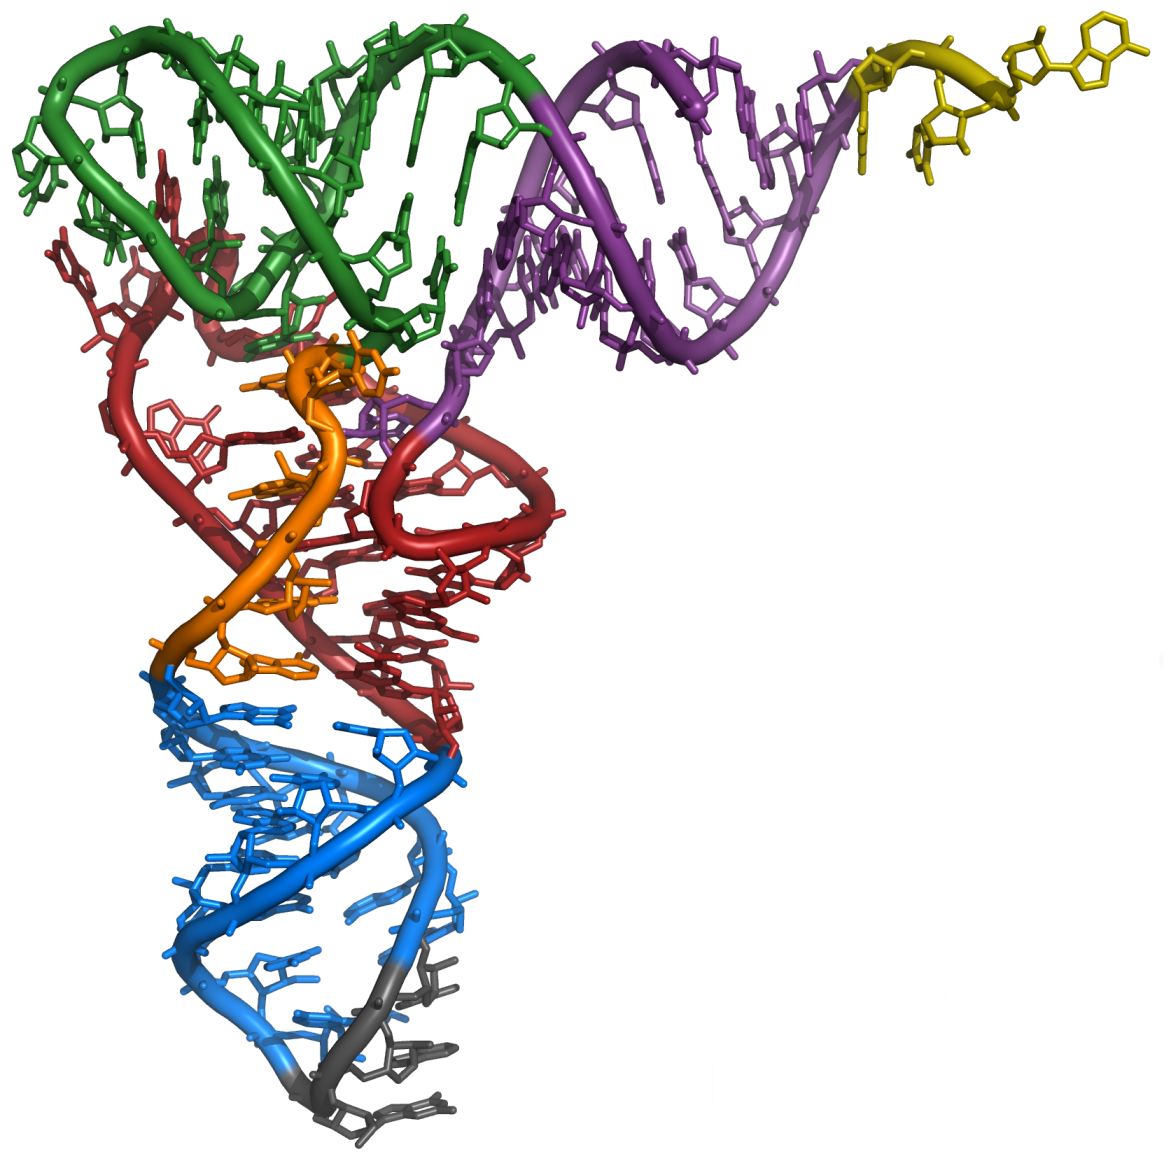
\includegraphics[scale=0.07]{trna}};
    %\node[name=tr,anchor=north west] at (16.3,9.50){\includegraphics[angle=90,origin=c,scale=.4]{crystal}};
    %
    \node[name=tr,anchor=north west] at (17.8,1.0){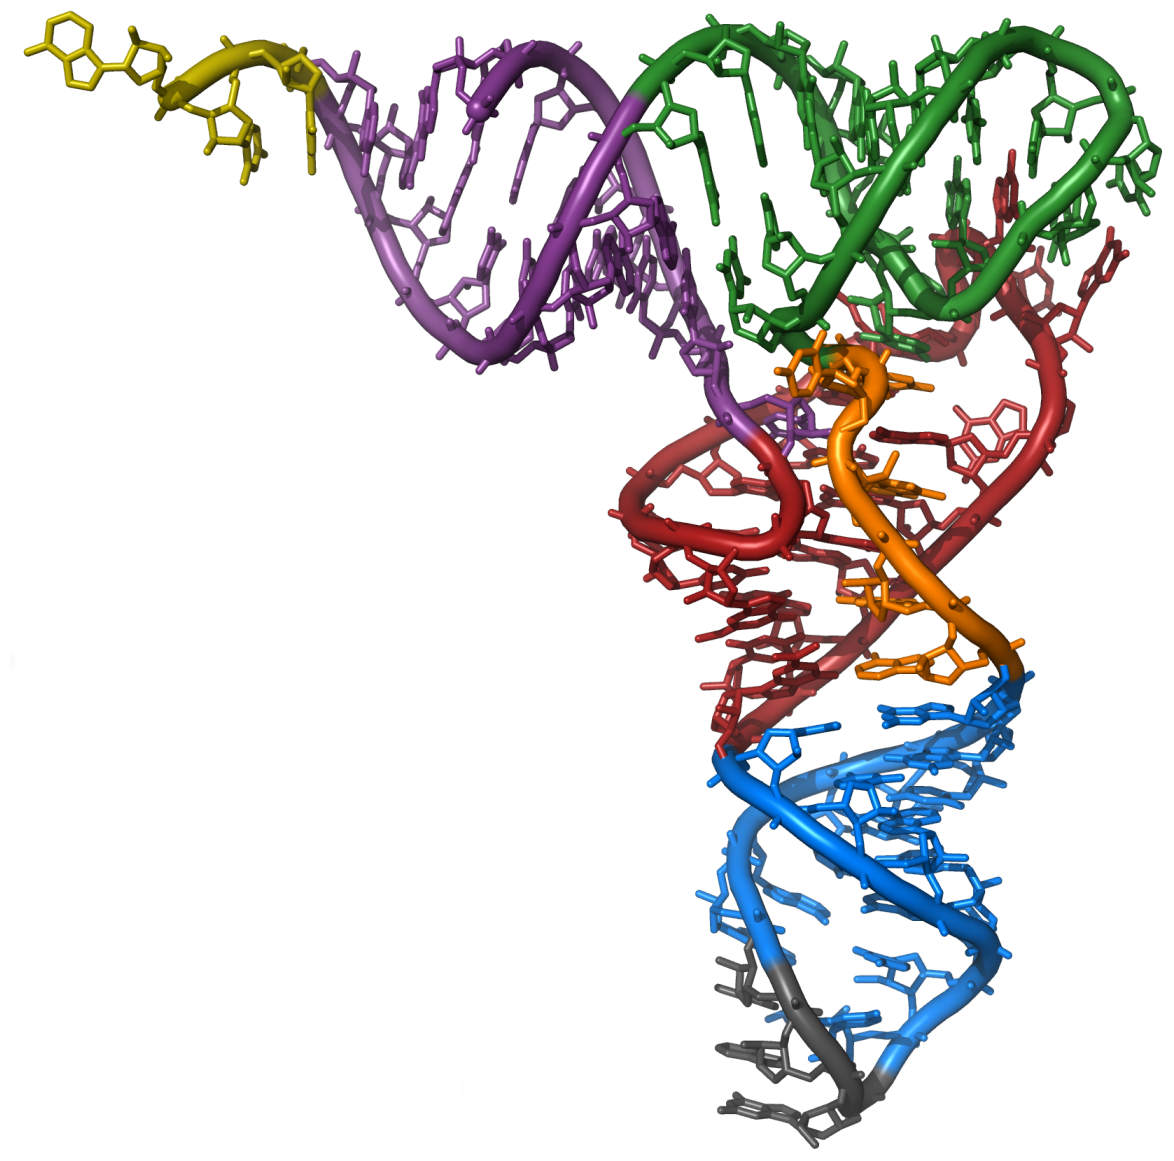
\includegraphics[scale=0.07]{trna2}};    %\node[name=tr,anchor=north west] at (18.5,0.850){\pgfornament[width=2cm,color=maroon,]{trna}};
   %\node[name=tr,anchor=north west] at (-7.9,-22.5){\includegraphics[scale=0.4]{sun}};
   %\node[name=tr,anchor=north west] at (17.5,-23.99){\includegraphics[angle=72,origin=c,scale=0.4]{05}};

%    \node[name=tr,anchor=north west] at (-0.55,-24.65){\pgfornament[width=2cm,color=maroon,symmetry=h]{131}};

     \node[name=tr,anchor=north west] at (-0.75,-23.95){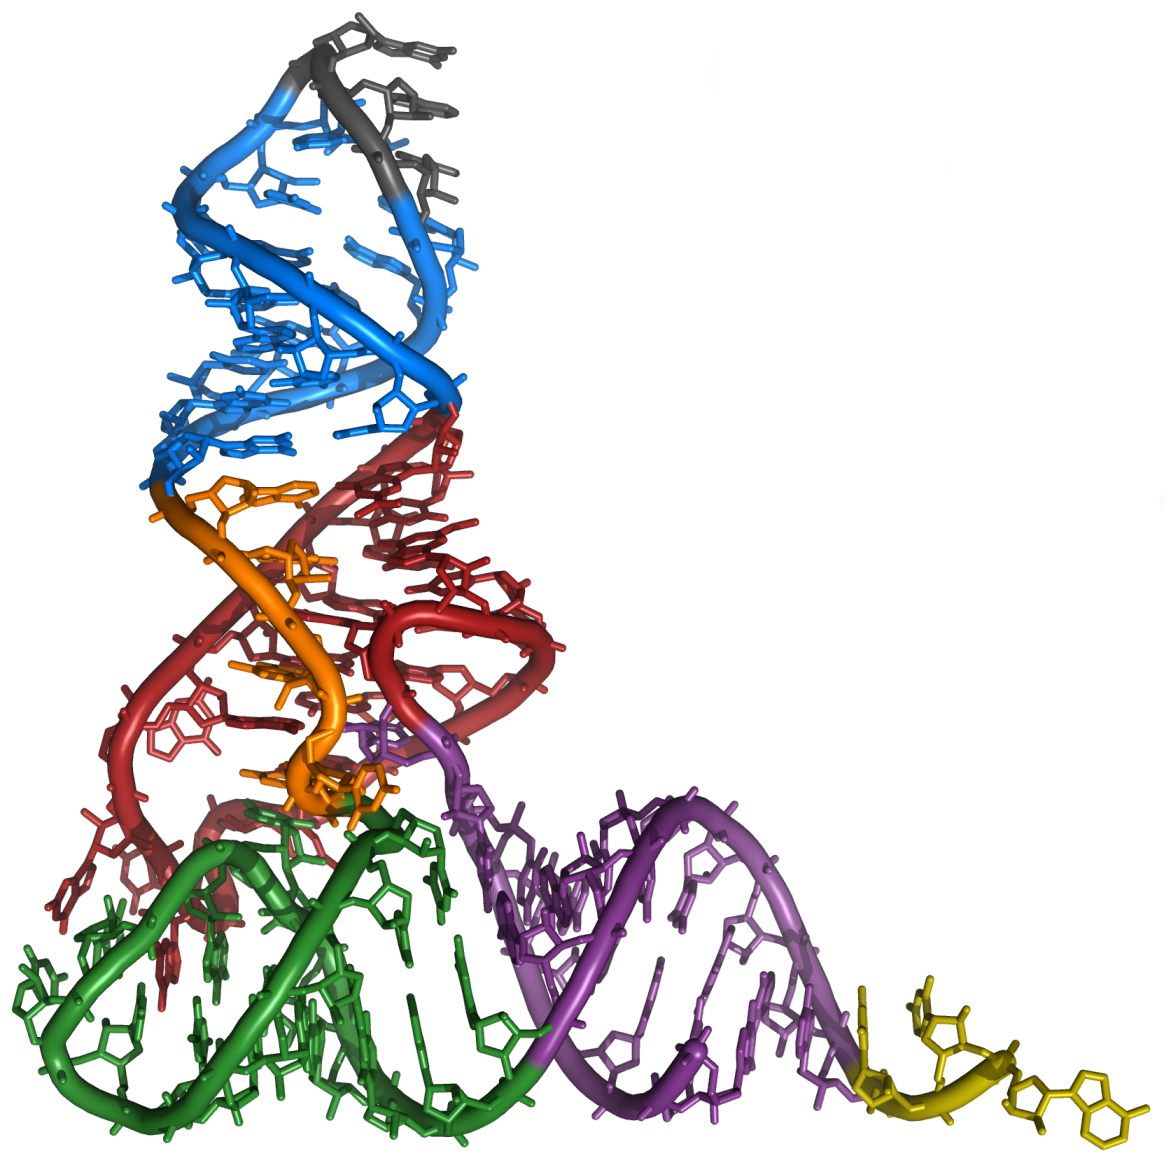
\includegraphics[scale=0.07]{trna4}};

     \node[name=tr,anchor=north west] at (17.8,-23.95){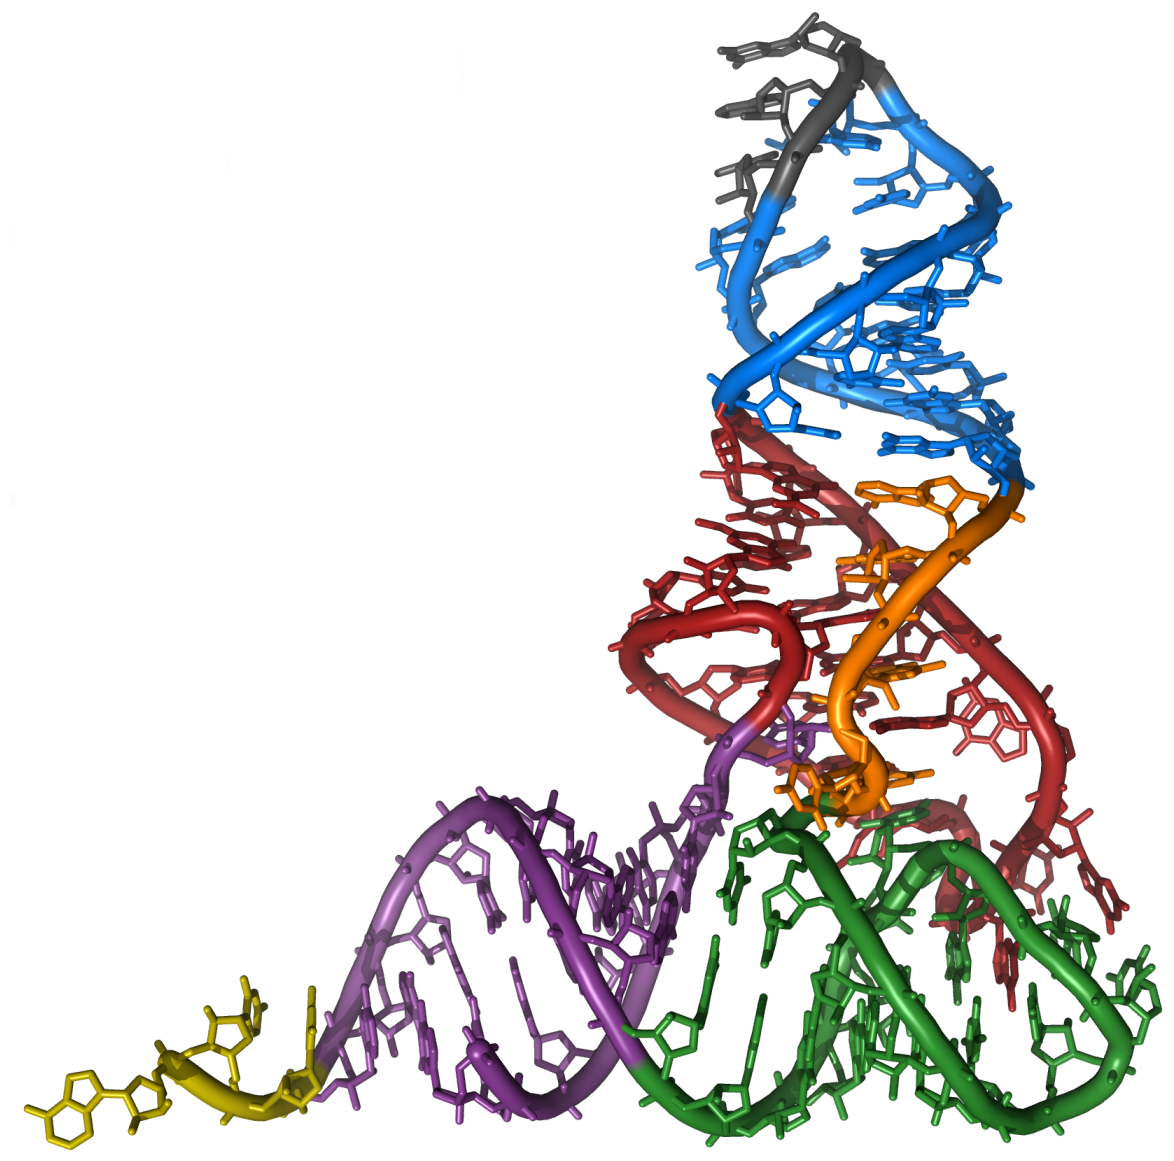
\includegraphics[scale=0.07]{trna3}};

%    \node[name=tr,anchor=north west] at (18.5,-24.65){\pgfornament[width=2cm,color=maroon,symmetry=h]{132}};
    \end{tikzpicture}

    \newpage
    \newgeometry{left=2.5cm,bottom=2.5cm,top=2.5cm,bottom=2.5cm}
    \begin{multicols}{2}
        \paragraph{\textsf{Abbreviations:}}
        \begin{itemize}
            \item \textbf{atm}: atmosphere
            \item \textbf{g, mg}: gram, milligram
            \item \textbf{K}: Kelvin
            \item \textbf{L, mL}: liter, milliliter
            \item \textbf{\textsc{M}}: Molar / molarity
            \item \textbf{mmHg}: millimeters of mercury
            \item \textbf{mol}: mole
        \end{itemize}
    \vspace{0.5cm}

    \paragraph{\textsf{Moles, conversion, pH, and other stuff : \newline}}

    \begin{itemize}
        \item 1 mole \( = \) \num{6.0221e23} things
        \item \( \textrm{Kelvin} = \si{\degreeCelsius} + \num{273.15} \)
        \item \( \textrm{\degree F} = 1.8 \times \si{\degreeCelsius} + \num{32} \)
        \item \( \si{\degreeCelsius} = \dfrac{(\textrm{\degree F} - \num{32})}{\num{1.8}} \)
        \item \( \textrm{pH} = \num{-1} \times  \log [\hydronium{}] \)
        \item \( \SI{1000}{\milli \liter} = \SI{1}{\liter} \)
        \item \( \grams{1000} = \SI{1}{\kilo \gram} \)
        \item \( \SI{1}{\milli \liter} = \SI{1}{\centi \meter \cubed} \)
        \item \( \SI{1000}{\calorie} = \SI{1}{\kilo \calorie} \)
        \item \( \text{density} = \dfrac{\text{mass}}{\text{volume}}\)
    \end{itemize}
\vspace{0.5cm}


\paragraph{\textsf{Concentration equations:}}

\begin{itemize}
    \item  \( \si{\pctmm}  = \dfrac{\text{mass of solute}}{\text{mass of solution}} \times \num{100}  \)
    \item \(\si{\pctvv} = \dfrac{\text{volume of solute}}{\text{volume of solution}} \times \num{100} \)
    \item \(\si{\pctmv}= \dfrac{\text{mass of solute in grams}}{\text{volume of solution in mL}} \times \num{100} \)
    \item Molarity \(= \dfrac{\text{number of moles of solute}}{\text{number of Liters of solution}}\)
\end{itemize}
\vspace{0.5cm}

\paragraph{\textsf{Gas equations:}}

\begin{itemize}
    \item \textbf{Boyle's Law}:    \( \mathrm{P_1 V_1} = \mathrm{P_2 V_2}  \)
    \item \textbf{Charles's Law}: \(\dfrac{\mathrm{V_1}}{\mathrm{T_1}} = \mathrm{\dfrac{V_2}{T_2}}\)
    \item \textbf{Gay-Lussac's Law}: \(\mathrm{\dfrac{P_1}{T_1} = \dfrac{P_2}{T_2}} \)
    \item \textbf{Combined gas Law}: \(\mathrm{\dfrac{P_1 V_1}{T_1} = \dfrac{P_2 V_2}{T_2}} \)
    \item \textbf{Avogadro's Law}: \( \mathrm{\dfrac{V_1}{n_1} = \dfrac{V_2}{n_2}} \)
    \item \textbf{Universal gas constant}: \( \mathrm{R} = \dfrac{\SI{0.0821}{\liter \atmosphere}}{\si{\mole \kelvin}}  \)
    \item \textbf{Ideal gas Law}: \( \mathrm{PV = nRT} \)
\end{itemize}
\end{multicols}
\end{document}


